\documentclass[xcolor=dvipsnames,hyperref={pdfpagelabels=false}]{beamer}

\usetheme{AnnArbor}

\let\Tiny=\tiny

\newcommand{\bi}{\begin{itemize}}
\newcommand{\ei}{\end{itemize}}
\newcommand{\be}{\begin{enumerate}}
\newcommand{\ee}{\end{enumerate}}
\newcommand{\bc}{\begin{center}}
\newcommand{\ec}{\end{center}}
\newcommand{\I}{\item}
\newcommand{\f}{\frame}
\newcommand{\ft}{\frametitle}
\newcommand{\newIcon}{
\includegraphics[width=0.2in]{new.jpg}}

\title{Hall D Data Flow and Data Challenges}
\subtitle{12 GeV Software Review, 2013}
\author[Mark M.\ Ito]{Mark M.\ Ito}
\date{November 25, 2013}
\institute[JLab]{Jefferson Lab}

\begin{document}

\f{\titlepage}

\section{Outline}

\f{\ft{Outline}
  \bi
  \I Data Flow, Computing Model
    \bi
    \I Raw data taking
    \I Reconstruction
    \I Analysis
    \I Simulation
    \ei
  \I Data Challenges, Past and Future~\newIcon
    \bi
    \I Offline Data Challenges
    \I Online Data Challenges
    \ei
  \ei
  \newIcon $\Rightarrow$ New since last review (June 2012)
}

\section{Data Flow}

\f{\ft{Raw data taking}
  \bi
  \I Detector to Level 3 Farm
    \bi
    \I Monitoring only at first
    \ei
  \I Farm to raid disk in Counting House
  \I EVIO format
  \I transfer to tape library
  \ei
}
\f{\ft{Reconstruction}
  \bi
  \I JANA framework
    \bi
    \I factory model: reconstructed objects on demand
    \I multi-threaded, event-level parallelization
      \bi
      \I scaling observed up to ??? cores
      \I thread memory footprint on the margin 30\% that of single-threaded job
      \ei
    \I calibration constants in relational database
    \ei
  \I REST formatted output~\newIcon
    \bi
    \I an HDDM: compressed XML
    \I compression from raw data: factor of 10
    \I self-documenting
    \I compact
    \ei
  \I Resource specification assumes all processing at JLab
    \bi
    \I Includes simulation
    \I Use Grid for unanticipated needs, large bursts
    \ei
  \ei
}
\f{\ft{Analysis}
  \bi
  \I Post-reconstruction options:~\newIcon
    \bi
    \I REST to Root Tree option
    \I REST to JANA option
    \ei
  \I Analysis Tools~\newIcon
    \bi
    \I user does not perform loops and sub-loops over particle combinations
    \I instead: specify reaction of interest (C++), including decays
    \I framework returns a list of combinations and their properties
    \I can request kinematic fits of various types
       \bi
       \I energy-momentum conservation
       \I mass constraints
       \I vertex constraints
       \ei
     \I already used in studies for PAC 40 proposal
       \bi
       \I demonstrated particle ID using only kinematics
       \ei
    \ei
  \ei
}
\f{\ft{Simulation}
  \bi
  \I on JLab Farm
  \I on the Grid
  \I geometry in XML (HDDS)
  \I using GEANT 3 based detector simulation
  \I conversion to Geant4 well-underway
    \bi
    \I use same geometry
    \I wrap hit generation from previous code base
    \I facilitate comparisons during transition
    \I overlaps eliminated in geometry~\newIcon
    \ei
  \ei
}
\section{Data Challenges}
  \subsection{Data Challenge I -- November/December 2012}
    \f{\ft{Data Challenge I: Goals}
      \bi
      \I produce and handle large data set
      \I look for issues in scaling
      \ei
    }
    \f{\ft{Data Challenge I: Configuration}
      \bi
      \I Minimum-bias hadronic events simulated, only coherent peak
      \I Events simulated and reconstructed in same job
      \I REST format reconstructed written to disk
      \I Simulated events discarded
      \I Sites:
        \bi
        \I Open Science Grid: peak 7000 jobs
        \I JLab Farm: peak 140 jobs
        \I Carnegie Mellon cluster: peak ??? jobs
        \ei
      \I Home-grown workflow tools, site-specific
        \bi
        \I Other tools seemed too heavy-weight and/or development would be needed
        \I Decision made to defer issue
        \ei
      \ei
    }
    \f{\ft{Data Challenge I: Results}
      \bi
      \I Event count: 5.4 billion events
        \bi
        \I Open Science Grid (OSG): 4.0 billion
        \I Jefferson Lab batch farm: 1.0 billion
        \I Carnegie Mellon Nuclear Physics Cluster: 0.4 billion
        \ei
      \I By event count: 2 weeks of data
      \I By usable data: 3 months of data
        \bi
        \I only generated coherent peak $\Rightarrow$ higher ``physics'' purity
        \ei
      \I Failure rate: about 7\%
        \bi
        \I hangs on single events
        \I segmentation faults
        \I corrupt output data
        \ei
      \ei
    }
    \f{\ft{Example Plot: $\gamma p\rightarrow\pi^+\pi^-\pi^0$}
      \bc
      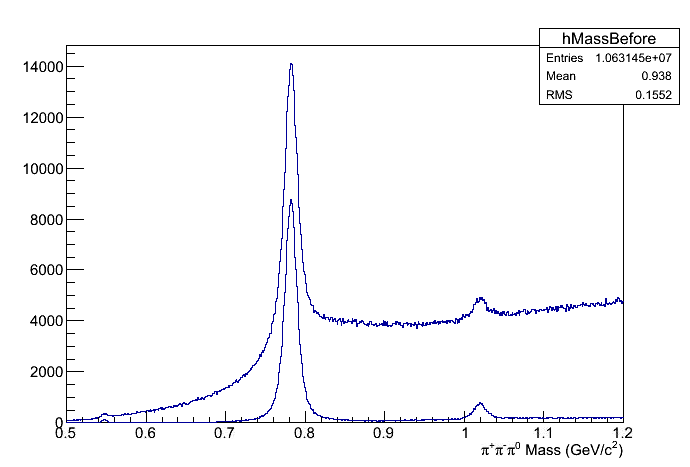
\includegraphics[width=3.4in]{omega_peak.png}
      \ec
      \bi
      \small
      \I 125 million events from DC I with particle ID cuts (2.4\% of total sample)
      \I shown with and without a cut on kinematic fit confidence level
        \bi
        \I cuts and fit performed with Analysis Tools
        \ei
      \ei
    }
\f{\ft{Data Challenge I: Lessons Learned}
      \bi
      \I Need to work hard on bullet-proofing the code
        \bi
        \I failures contribute to fraction of effort far greater than fraction of failures
        \ei
      \I Tools at JLab need development
        \bi
        \I JLab Scientific Computing Department may help here
        \ei
      \I Need a global (Grid + JLab) meta-data catalog
      \ei
    }
  \subsection{Online Data Challenge I -- August 2013}
    \f{\ft{Online Data Challenge I: Goals}
      \bi
      \I look for bandwidth bottlenecks
      \I measure performance of monitoring farm
      \I test level 3 algorithm
      \I transfer to tape library
      \ei
    }
    \f{\ft{Online Data Challenge I: Configuration}
      \bi
      \I Events pre-staged on disk
      \I Inserted to Event Transfer system (data buffer, supports multiple event producers, multiple event consumers)
      \I Transferred to Level 3 farm, ??? nodes
      \I Written to raid disk
      \I Transferred to tape library
      \ei
    }
    \f{\ft{Online Data Challenge I: Results}
      \bi
      \I Level 3 farm measured bandwidth 40 kHz, ??? MB/s
      \I SEST-to-EVIO conversion worked; reconstructible events
      \I RootSpy: collection of root objects (histograms) from multiple processes succeeded
      \I Others???
      \ei
    }
    \f{\ft{Level 3 Farm Throughput}
      \begin{columns}[c]
        \begin{column}{1.6in}
          \small
          \bi
          \I Adding ten nodes to the farm, one by one
            \bi
            \I two $\times$ 2.5~GHz Intel Xeon (8~cores, 16~hyperthreads)
            \I eight $\times$ 1.9~GHz AMD Opteron (8~cores)
            \ei
          \ei
        \end{column}
        \begin{column}{2.9in}
          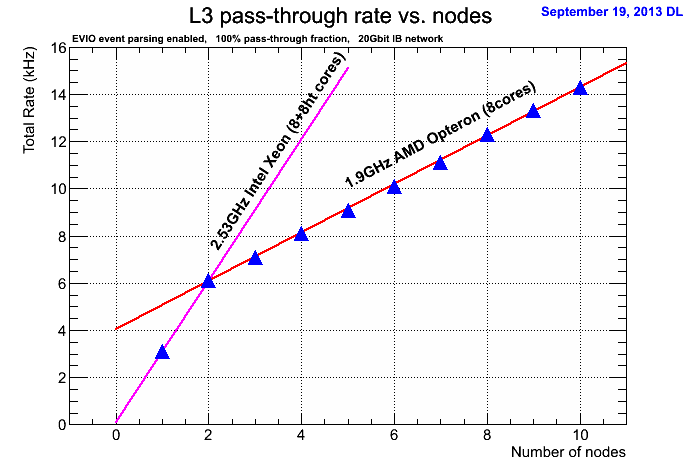
\includegraphics[width=2.9in]{cpu_scaling.png}
        \end{column}
      \end{columns}
      \bi
      \small
      \I Nodes mostly borrowed from IT Division
      \I Unpacking only: creation of C++ data objects, including translation from geographic to logical addresses
      \I Data ready-to-analyze, but no analysis done
      \I All 10 nodes: 14 kHz, still CPU limited
      \ei
    }
    \f{\ft{Online Data Challenge I: Lessons Learned}
      \bi
      \I Counting room to tape library transfer should not use standard command-line tool (solved: SciComp method implemented, tested)
      \I Simple unpacking saturated CPU with nodes used
      \I Initial Hall D Farm (now installed) can keep up with execution of Level 3 at intensity $10^7\ \gamma$/s
      \ei
    }
  \subsection{Future Data Challenges}
    \f{\ft{Data Challenge II -- December 2013}
      \bi
      \I Goals
        \bi
        \I 10 giga-events
        \I EM background
        \I modern reconstruction
        \ei
      \I Status -- ongoing mini-challenges
      \ei
    }
    \f{\ft{Online Data Challenge II - January 2014}
      \bi
      \I Goals
        \bi
        \I End-to End test
        \I events will start in front-end electronics crates
        \I transfer to tape library will use production method
        \ei
      \I Status -- preparations underway
      \ei
    }
    \f{\ft{Data Challenge III - February 2014}
      \bi
      \I Two-step process
        \bi
        \I event generation in one set of jobs
        \I reconstruction in independent set of jobs
        \ei
      \I exercises raw data analysis mode
      \I less efficient, may re-use ``raw'' data sets
      \ei
    }
\section{Conclusions}

  \f{\ft{Conclusions}
    \bi
    \I Data Flow plan has remained stable
    \I Addition of REST format since last review
    \I Series of Data Challenges Performed and Planned
      \bi
      \I Done: DC1, ODC1
      \I In preparation: DC2, ODC2, DC3
      \ei
    \I Involvement of IT Division's Scientific Computing Group in collaborative development of workflow/provenance tools
    \I On track to be ready for data taking
    \ei
  }

\end{document}

% end of latex file
